\documentclass{article}

\usepackage{graphicx}
\usepackage{tikz}
\usepackage{tikzsymbols}
\usetikzlibrary{calc,patterns,shapes.geometric}
\pagestyle{empty}
\usepackage[margin=0pt]{geometry}
\geometry{papersize={14in,12in}}

\def\centerarc[#1](#2)(#3:#4:#5){\draw[#1] ($(#2)+({#5*cos(#3)},{#5*sin(#3)})$) arc (#3:#4:#5);}

\begin{document}
	\begin{figure}
		\centering
		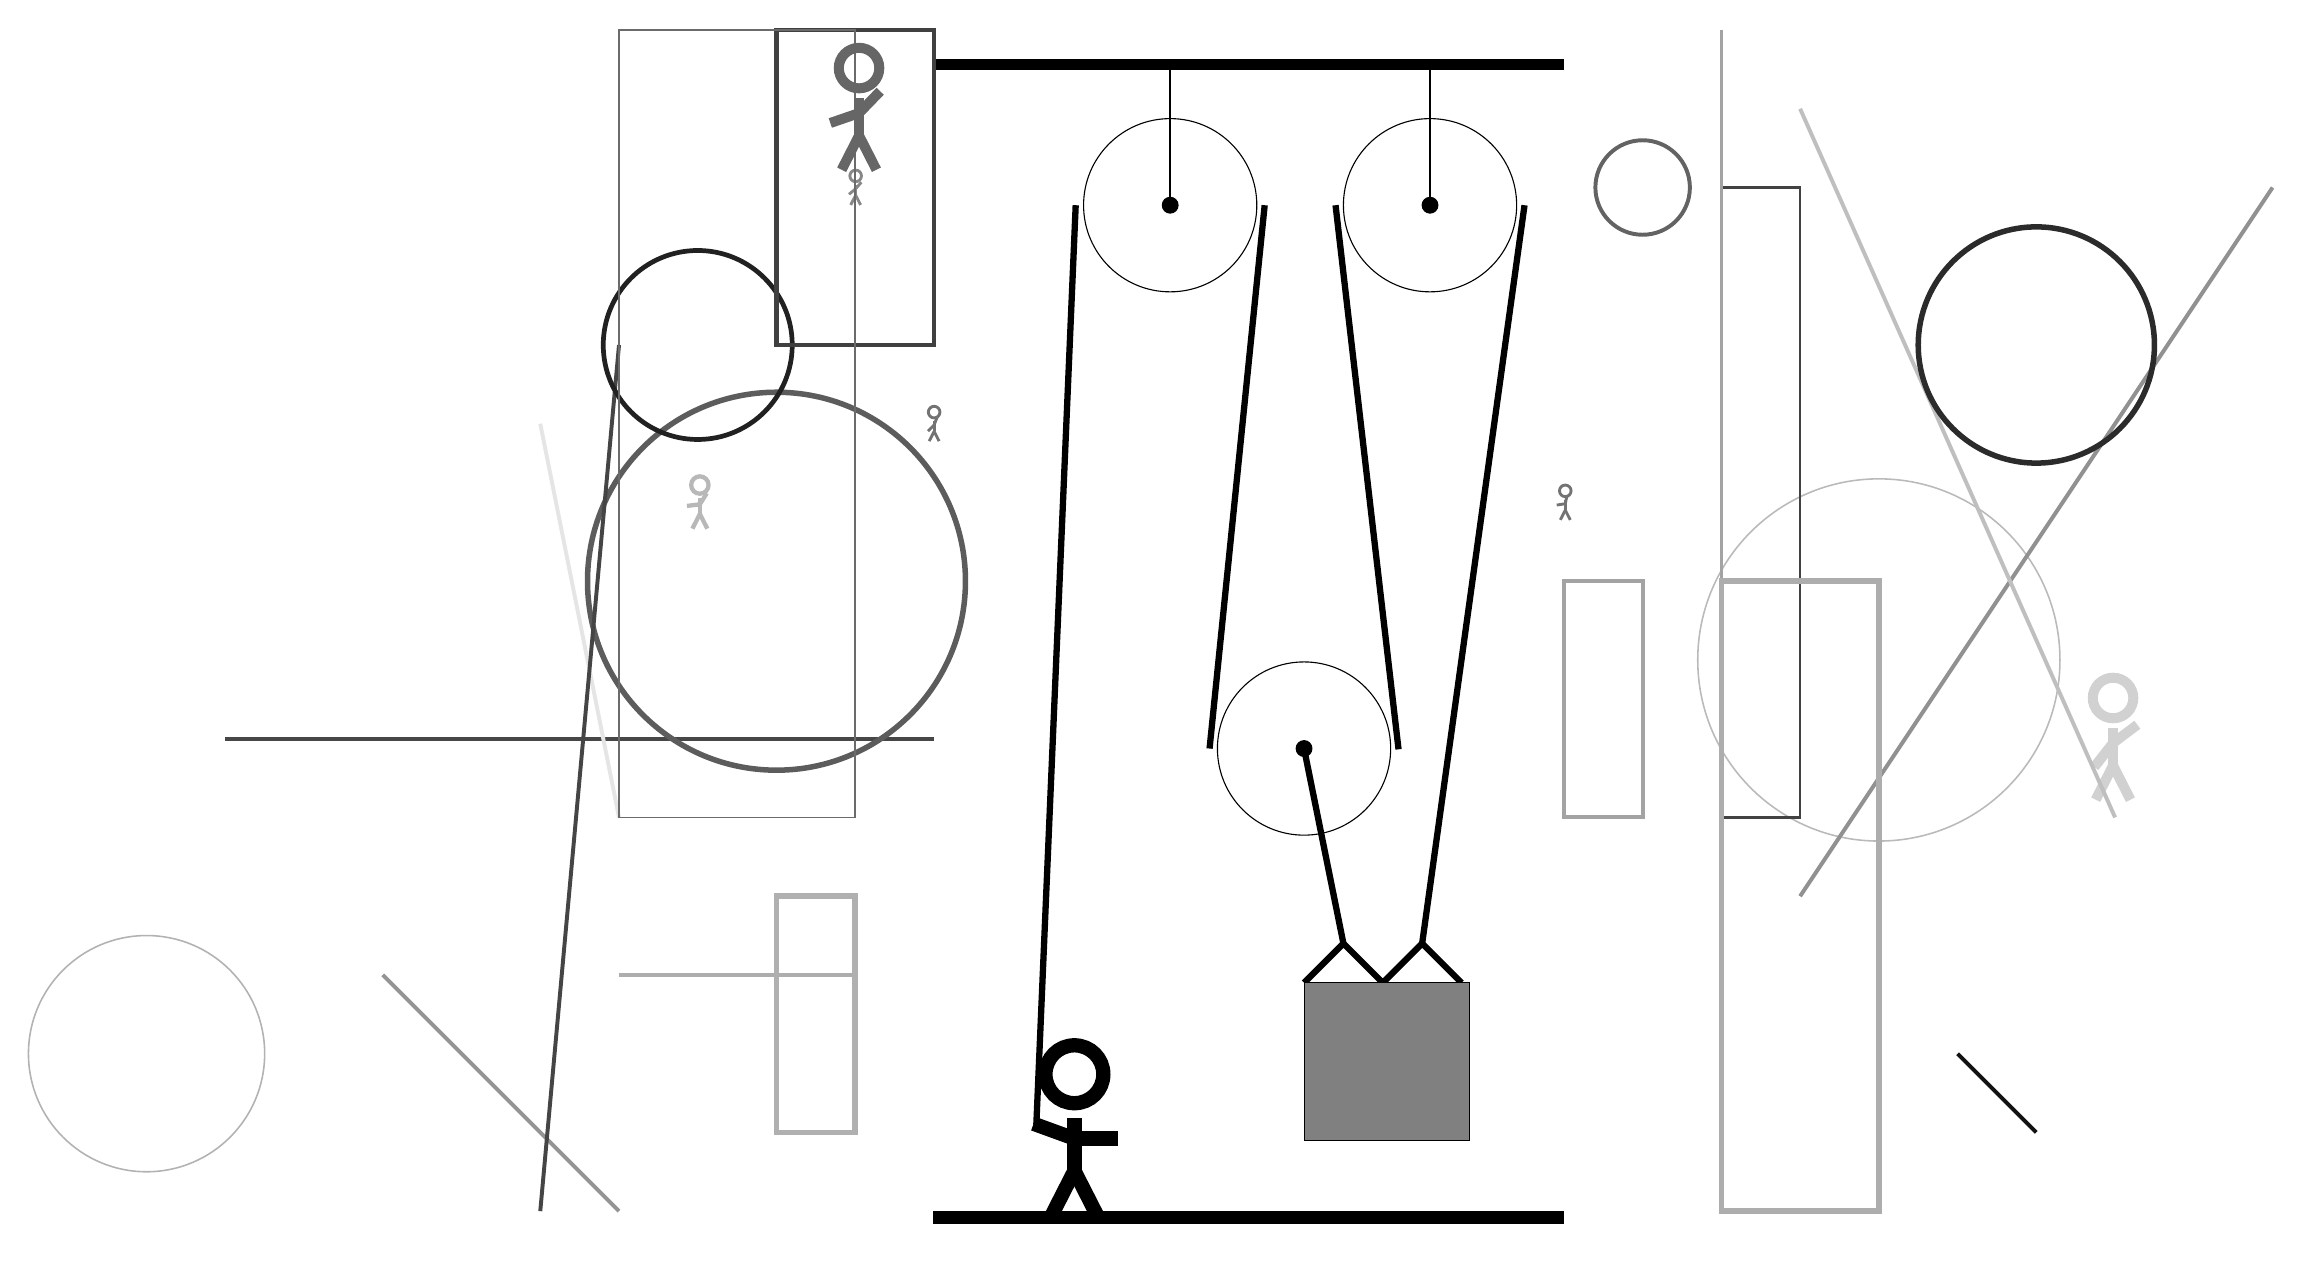
\begin{tikzpicture}
			%%%%% START %%%%%
			
			\draw[fill=black] (-2, 11.5) rectangle (6, 11.625);
			
			\draw (1, 9.775) circle (1.1);
			\draw[fill=black] (1, 9.775) circle (0.1);
			\draw[thick] (1, 9.775) -- (1, 11.5);
			
			\draw (4.3, 9.775) circle (1.1);
			\draw[fill=black] (4.3, 9.775) circle (0.1);
			\draw[thick] (4.3, 9.775) -- (4.3, 11.5);
			
			\draw [line width=0.2mm, color=black!27](10, 4) circle (2.3);
			
			\draw[line width=0.5mm, color=black!93](11, -1) -- (12, -2);
			\draw[line width=0.5mm, color=black!72](-2, 3) -- (-11, 3);
			\draw[line width=0.5mm, color=black!10](-7, 7) -- (-6, 2);
			\node[line width=0.5mm, color=black!28] at (-5, 6) {\Strichmaxerl[3][7][58]};
			\draw[line width=0.5mm, color=black!32](-6, 0) -- (-3, 0);
			
			\node[line width=0.4mm, color=black!55] at (-2, 7) {\Strichmaxerl[2][45][69]};
			
			\draw[line width=0.3mm, color=black!74] (8, 10) rectangle (9, 2);
			\draw [line width=0.7mm, color=black!64](-4, 5) circle (2.4);
			\node[line width=0.5mm, color=black!18] at (13, 3) {\Strichmaxerl[7][52][37]};
			
			\draw[line width=0.5mm, color=black!42](-6, -3) -- (-9, 0);
			\draw[line width=0.5mm, color=black!43](9, 1) -- (15, 10);
			\draw[line width=0.5mm, color=black!73](-6, 8) -- (-7, -3);
			
			\draw [line width=0.6mm, color=black!87](-5, 8) circle (1.2);
			\node[line width=0.5mm, color=black!47] at (-3, 10) {\Strichmaxerl[2][40][49]};
			\draw[line width=0.5mm, color=black!36] (7, 5) rectangle (6, 2);
			\draw[line width=0.5mm, color=black!25](9, 11) -- (13, 2);
			\draw[line width=0.7mm, color=black!31] (-3, 1) rectangle (-4, -2);
			\draw[line width=0.3mm, color=black!36] (8, 12) rectangle (8, -1);
			
			\draw[line width=0.6mm, color=black!75] (-2, 8) rectangle (-4, 12);
			\node[line width=0.6mm, color=black!55] at (6, 6) {\Strichmaxerl[2][9][78]};
			\draw [line width=0.2mm, color=black!30](-12, -1) circle (1.5);
			\draw[line width=0.2mm, color=black!58] (-3, 2) rectangle (-6, 12);
			\draw [line width=0.7mm, color=black!83](12, 8) circle (1.5);
			\node[line width=0.2mm, color=black!60] at (-3, 11) {\Strichmaxerl[7][19][46]};
			\draw [line width=0.5mm, color=black!61](7, 10) circle (0.6);
			
			\draw[line width=0.7mm, color=black!32] (8, -3) rectangle (10, 5);
			
			\draw (2.7, 2.875) circle (1.1);
			\draw[fill=black] (2.7, 2.875) circle (0.1);
			
			\draw[line width=0.8mm]  (2.7, -0.1) -- (3.2, 0.4) -- (3.7, -0.1) -- (4.2, 0.4) -- (4.7, -0.1);
			\draw[fill=black!50] (2.7, -0.1) rectangle (4.8, -2.1);
			
			\draw[line width=0.8mm](-0.7, -1.9) -- (-0.2, 9.775);
			\centerarc[line width=0.8mm](1, 9.775)(0:180:1.2000000000000002);
			\draw[line width=0.8mm](2.2, 9.775) -- (1.5, 2.875);
			\centerarc[line width=0.8mm](2.7, 2.875)(180:370:1.2000000000000002);
			\draw[line width=0.8mm] (3.9, 2.865) -- (3.1, 9.775);
			\centerarc[line width=0.8mm](4.3, 9.775)(0:180:1.2000000000000002);
			\draw[line width=0.8mm](4.2, 0.4) -- (5.5, 9.775);
			\draw[line width=0.8mm] (3.2, 0.4) -- (2.7, 2.875);
			
			\node at (-0.2, -2) {\Strichmaxerl[10][-20][0]};
			
			\draw[fill=black] (-2, -3) rectangle (6, -3.15);
			
			%%%%% END %%%%%
		\end{tikzpicture}
	\end{figure}	
\end{document}